% $Id: testresultprefs.tex 12292 2010-09-23 12:45:32Z alexandra $
% Local Variables:
% ispell-check-comments: nil
% Local IspellDict: american
% End:
% --------------------------------------------------------
% User documentation
% copyright by BREDEX GmbH 2005
% --------------------------------------------------------
\index{Preferences!Test Result}
\index{Test Result!Preferences}
\index{XML and HTML Result Reports}
\index{Results!XML and HTML Reports}



\begin{figure}[h]
\begin{center}
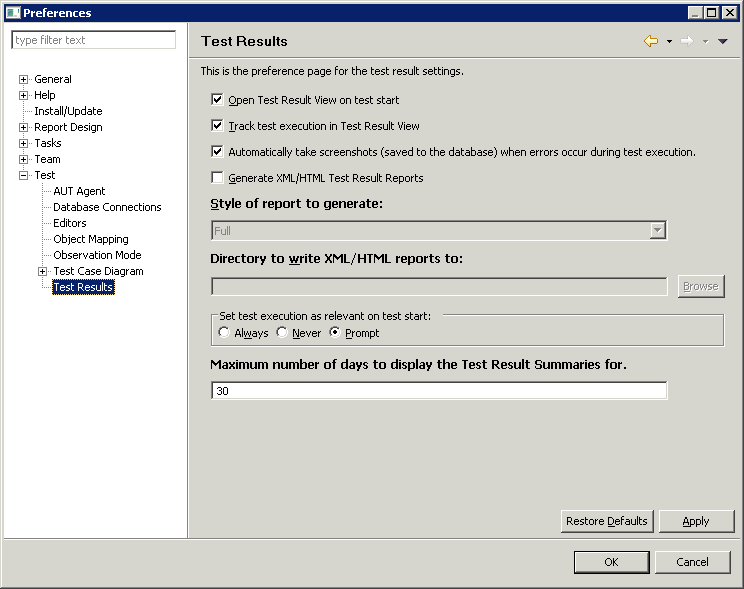
\includegraphics[width=12.5cm]{Tasks/Preferences/PS/testresultprefs}
\caption{Test Result Preference Dialog}
\label{testresultprefs}
\end{center}
\end{figure}
\begin{enumerate}
\item Choose whether you want the  \gdtestresultview{} to open when testing begins. 

The \gdtestresultview{} follows the test execution and shows which \gdsteps{} were successful and which failed. 

\item Choose whether you want to track the test execution progress in the \gdtestresultview{}. When this option is activated, the \gdtestresultview{} scrolls to follow the test progress. 
\item Choose whether you want to create HTML and XML reports for each execution. When you activate this choice, decide whether you want full reports or just the errors to be shown. Enter a directory for the reports. 
\item Choose whether you want \app{}to automatically create a screenshot when a test encounters an error. Screenshots are automatically saved in the \gddb{} and can be viewed using the \gdimgview{} when you select the failed \gdstep{} in the \gdtestresultview{}. 
\item Decide whether you want all test runs or no test runs to be marked as relevant, or whether you want to be prompted each time. If a test run is marked as non-relevant, then it will not be included for any generated BIRT reports, nor will it be exported when the \gdproject{} is exported. 
\end{enumerate}


